\documentclass[12pt,letterpaper]{article}
%\usepackage{preamble}

%\ProvidesPackage{preamble}

\usepackage{fullpage}
\usepackage[top=2cm, bottom=4.5cm, left=2.5cm, right=2.5cm]{geometry}
\usepackage{amsmath,amsthm,amsfonts,amssymb,amscd}
\usepackage{lastpage}
\usepackage{enumerate}
\usepackage{fancyhdr}
\usepackage{mathrsfs}
\usepackage{xcolor}
\usepackage{graphicx}
\usepackage{listings}
\usepackage{hyperref}
\usepackage{enumitem}
\usepackage{float}
\usepackage{fancyvrb}
\usepackage{color,soul}
\sethlcolor{lightgray}
 \usepackage{subfigure}
 \usepackage{textcomp}
\usepackage{siunitx}

\usepackage{graphicx}
\usepackage{array}

\usepackage[T1]{fontenc}
\usepackage[numbered,framed]{matlab-prettifier}
\hypersetup{%
  colorlinks=true,
  linkcolor=blue,
  linkbordercolor={0 0 1}
}

\let\ph\mlplaceholder % shorter macro
\lstMakeShortInline"

\lstset{
  style              = Matlab-editor,
  basicstyle         = \mlttfamily \small,
  escapechar         = ",
  mlshowsectionrules = true,
  xleftmargin=.01\textwidth, xrightmargin=.01\textwidth
}

\graphicspath{{./problem1_images}}

\pagestyle{fancyplain}
\headheight 35pt
\lhead{\userID}
\chead{\textbf{\Large Project \hwnumber}}
\rhead{\course \\ \today}
\lfoot{}
\cfoot{}
\rfoot{\small\thepage}
\headsep 1.5em




%%%%%%%%%%%%%%%%%%%%%%%%%%%%%%%%%%%%%%%%%%
%%%% Edit These for yourself
%%%%%%%%%%%%%%%%%%%%%%%%%%%%%%%%%%%%%%%%%%
\newcommand\course{Econ 672}
\newcommand\hwnumber{}
\newcommand\userID{Ziming Huang}
\newenvironment{alphaparts}[0]{%
  \begin{enumerate}[label=\textbf{\Alph*}]
}{\end{enumerate}}


\begin{document}
\section*{Question 0}
We will use these stocks to solve Question 1 to 3.

\begin{table}[ht]
%\caption{ Estimated IV for September 15, 2008 (using TV)} % title of Table
\centering % used for centering table
\begin{tabular}{c c} % centered columns (4 columns)
\hline\hline %inserts double horizontal lines
Stock & Ticker\\ [0.5ex] % inserts table
%heading
\hline % inserts single horizontal line
1 & PG \\ % inserting body of the table
2 & DIS \\ %[1ex] % [1ex] adds vertical space
3 & SPY \\
\hline %inserts single line
\end{tabular}
\end{table}
\vspace{-6mm}

\section*{Question 1}
  \begin{enumerate}[label=\textbf{(\Alph*)}]
%----A-----
\item
\begin{enumerate}[label=(\roman*)]
\item In our data set, September 16, 2008 is the 430$_{th}$ observation day, so $t(September 16,2008)=430$.

%\item The value of ${t}$ here is the date of available historical data. If we want to calculate today's IV but today's market data is not available, we may need to use yesterday's data to do forecasting for today's IV, in this case ${t}$ will exactly equal to the last trading day: September 15, 2008 (Specifically, for our data set, September 15, 2008 is the 430th observation day, so for log-returns, ${r_t^c} = r_{429}^c$). 

%\vspace{0.9mm}
%Or if today's market hours are over, we can still use today's data to calculate our statistics, then $t$ here can be September 16, 2008.

\item It is not possible to use today's data to estimate today's IV, since it is the morning now, we do not have enough price data to do this estimation. However, we can use the historical data to estimate today's IV by doing forecasting.
 \end{enumerate}
 
 
%----B-----
\item The follow is the estimated value of IV in September 15, 2008.
\begin{table}[ht]
%\caption{ Estimated IV for September 15, 2008 (using TV)} % title of Table
\centering % used for centering table
\begin{tabular}{c c} % centered columns (4 columns)
\hline\hline %inserts double horizontal lines
Stock & Estimated IV of September 15, 2008(using TV)\\ [0.5ex] % inserts table
%heading
\hline % inserts single horizontal line
PG &  $2.2430\times 10^{-4}$  \\ % inserting body of the table
DIS & $4.9671\times 10^{-4}$ \\ %[1ex] % [1ex] adds vertical space
\hline %inserts single line
\end{tabular}
\end{table}
\vspace{-6mm}

\begin{enumerate}[label=(\roman*)]
\item Since there are jumps existing in stock price, to better estimate the value of IV, we here choose truncated variance as a estimator for IV. This value measures the intraday fluctuation in stock's price: the bigger value of estimated IV, the more volatility we will expected for stock's price. From this table, the DIS' $IV_t$ is larger than PG's, which means the price(or return) volatility of DIS is bigger than PG's, that is, DIS' stock is more risky.

\item The reason we use the historical (yesterday) data to  do forecasting for today's IV is that: the history data reflects the information of a company, this information includes its financial performance, financial position and operation strategy. Besides, the history data also contain the relationship between the company and the market environment, such as market interest, CPI index and other micro-structure shocks. This information is really important for us to understand and evaluate a company. Since a company's structure and relationship between market will not change in a short time, it is reasonable for us to believe that the recent history data can reflect company's status well so it can be use to do future forecasting. (we still need to think carefully whether this assumption holds or not: the future data shares the same distribution of historical data. Only under this assumption can we regard historical data as a good estimator for future statistics and these forecasts will be efficient).  
 \end{enumerate}
 %----C-----
 \item 
 To calculate the loss probability, we follow these steps:
 \begin{enumerate}[label=(\roman*)]
 \item Estimate the parameter ${IV_t}$ in the $r_t^c$ 's asymptotic distribution $\mathcal{N}(0,IV_t)$ by truncated variance $TV_t$;
 \item Standardize $r_t^c$ and compute the loss probability by using the CDF of standard normal distribution:
 $$\frac{r_t^c}{\sqrt{IV_t}}=Z_t \sim \mathcal{N}(0,1)$$
 $$\mathbb{P}(r_t^c <= -q)=\mathbb{P}(\frac{r_t^c}{\sqrt{IV_t}}<=\frac{-q}{\sqrt{IV_t}})=\mathbb{P}(Z_t<=\frac{-q}{\sqrt{IV_t}})=1-\Phi(\frac{q}{\sqrt{IV_t}})$$
 \end{enumerate}
 
 By replacing q=2\% (or 4\%) and $\hat{IV_t}=TV_{yesterday}$, we can compute the loss probability.\\
 \vspace{5mm}
 
 To calculate the $CI(IV_{t})$ and $CI(\mathbb{P})$, we follow these steps:
 \begin{enumerate}[label=(\roman*)]
 \item Compute $CI(\Delta_n^{-0.5}(TV_t-IV_t))$ from its asymptotic distribution:
 $$\Delta_n^{-0.5}(TV_t-IV_t) \xrightarrow{d}  \mathcal{N}(0,2QIV_t)$$
 $$\Rightarrow  ~~~~CI(\Delta_n^{-0.5}(TV_t-IV_t))=[-c\sqrt{2QIV_t},~~ c\sqrt{2QIV_t}~]$$
 \item Deduce the $CI(IV_t)$ 's expression from $CI(\Delta_n^{-0.5}(TV_t-IV_t))$  :
$$CI(IV_t,c)=[-c\sqrt{2\Delta_n QIV_t}+TV_t, ~~c\sqrt{2\Delta_n QIV_t}+TV_t ]$$
 
\item Estimate parameter $QIV_t$ and compute the CI of $IV_t$:
\vspace{-1mm}
 $$\hat{QIV_t}=\frac{1}{3 \Delta_n}\sum_{i=1}^{n}(r_{t,i}^c)^4$$
 \vspace{-1mm}
 $$CI(IV_t)=[-c\sqrt{2\Delta_n\hat{QIV_t}}+TV_t,~~ c\sqrt{2\Delta_n\hat{QIV_t}}+TV_t ]$$
 
 where $c$ is the critical value and equals $\Phi(1-\frac{0.05}{2})=1.96$ in this case (95\% significant level).

\item Use $CI(IV_t$) 's upper bound and lower bound as new variance in $r_t^c$ 's asymptotic distribution to calculate $CI(\mathbb{P})$:
$$CI^{up}(\mathbb{P})=\mathbb{P}(r_t^c <= -q)=\mathbb{P}(Z_t<=\frac{-q}{\sqrt{IV_t^{upper}}})=1-\Phi(\frac{q}{\sqrt{IV_t^{upper}}})$$
\vspace{-3mm}
$$CI^{low}(\mathbb{P})=\mathbb{P}(r_t^c <= -q)=\mathbb{P}(Z_t<=\frac{-q}{\sqrt{IV_t^{lower}}})=1-\Phi(\frac{q}{\sqrt{IV_t^{lower}}})$$
 \end{enumerate}
By replacing q=2\% (or 4\%), we can compute the $CI(\mathbb{P})$.
\newpage

\begin{table}[ht]
\centering % used for centering table
\begin{tabular}{c c c c c} % centered columns (4 columns)
\hline\hline %inserts double horizontal lines
& & \multicolumn{3}{c}{Estimate of $\mathbb{P}(r_t^c <= -q)$}\\ [0.5ex]%inserts table
\cline{3-5} Stock & q & Estimate & Lower bound & Upper bound\\ 
%heading
 % inserts single horizontal line
 \hline
PG & 2\% & 0.0909 & 0.0404 & 0.1308 \\ % inserting body of the table
PG & 4\% & 0.0038 & $2.3953\times 10^{-4}$ & 0.0124 \\ %[1ex] % [1ex] adds vertical space
DIS & 2\% & 0.1848 & 0.1392& 0.2169 \\ % inserting body of the table
DIS & 4\% & 0.0363 & 0.0151 & 0.0588 \\
\hline %inserts single line
\end{tabular}
\end{table}

According to the table, we can find that the width of confidence interval is in the range 0.01-0.09, which means the biggest difference between real probability of losing certain amount of money and the estimated probability will be 9 percentage. This outcome isn't very accuracy. However, given that confidence intervals' width of losing 4\% money  fall in the range 0.1-0.4, this estimated confidence interval may be accuracy in this case. 

%-----------part D
\item To compute the VaR and its confidence interval, we follow these steps:
\begin{enumerate}[label=(\roman*)]
    \item Transfer the asymptotic distribution of $r_t^c$ to standard normal distribution:
     $$\frac{r_t^c}{\sqrt{IV_t}}=Z_t \sim \mathcal{N}(0,1)$$
\item Compute the loss probability by the CDF of standard normal distribution(here ${r_t^c ~\%}$ is the percentage log return):
     $$\mathbb{P}(\frac{r_t^c ~\%}{100}\times V<= Q)=\mathbb{P}({r_t^c ~\%}<=\frac{100Q}{V})=\Phi(\frac{100Q}{V\sqrt{IV_t}})=p$$
\item Compute the value of Q by taking inverse to the  CDF of standard normal distribution:
    $$Q=\Phi^{-1}(p)\frac{V\sqrt{IV_t}}{100}$$
\item(\emph{Delta Method}) Since we have already known the asymptotic distribution of $\Delta_n^{-0.5}(TV_t-IV_t)$, we can apply Delta Method to deduce the asymptotic distribution of $Q$ and then use it to compute $CI(Q)$:

$$\Delta_n^{-0.5}(\sqrt{TV_t}-\sqrt{IV_t}) \xrightarrow{d} \mathcal{N}(0,2QIV_t)$$
$$Delta ~Method \Rightarrow ~~ \Delta_n^{-0.5}\Phi^{-1}(p)\frac{V}{100}(\sqrt{TV_t}-\sqrt{IV_t}) \xrightarrow{d} \mathcal{N}(0,\frac{QIV_t}{2IV_t})$$

\vspace{3mm}

so the confidence interval of Q is:

\vspace{-3mm}

$$CI^{up}(Q,1-\alpha)=\Phi^{-1}(p)\frac{V}{100}(\sqrt{TV_t}) + c \ast \Phi^{-1}(p)\frac{V}{100}\sqrt{\frac{\hat{\Delta_n QIV_t}}{2TV_t}}~$$

\vspace{-5mm}

$$CI^{low}(Q,1-\alpha)=\Phi^{-1}(p)\frac{V}{100}(\sqrt{TV_t}) - c \ast \Phi^{-1}(p)\frac{V}{100}\sqrt{\frac{\hat{\Delta_n QIV_t}}{2TV_t}}~$$

\begin{table}[ht]
%\caption{ Estimated IV for September 15, 2008 (using TV)} % title of Table
\centering % used for centering table
\begin{tabular}{ccccc} % centered columns (4 columns)
\hline\hline %inserts double horizontal lines
\multicolumn{5}{c}{VaR Estimate and 95\% Confidence interval}\\
\hline Stock & p & Estimate & Lower bound & Upper bound\\
%heading
\hline % inserts single horizontal line
PG & 1\% & -6.9681 & -5.5126 & -8.4236 \\ % inserting body of the table
PG & 5\% & -4.9268 & -3.8977 & -5.9560 \\ %[1ex] % [1ex] adds vertical space
DIS & 1\% & -10.3694 & -8.7269 & -12.0119 \\ % inserting body of the table
DIS & 5\% &-7.3318 & -6.1704 & -8.4931\\
\hline %inserts single line
\end{tabular}
\end{table}
\newpage
According to the table, we can find that the width of confidence interval is in the range 2.0~-~3.3. To cancel the effect of scale, it is much better to use percentage width to evaluate the accuracy of confidence interval. In thus case, the percentage width of confidence interval is in the range of 1.00\%~-~1.65\%, so the level of accuracy is sufficient and my boss may find them helpful.\\
    
(Simplified) 

We can also use $CI^{up}(IV_t)$ and $CI^{low}(IV_t)$ as new variance to compute $Q$. These two values of Q will be our $CI^{up}(Q)$ and $CI^{low}(Q)$:

\vspace{-3mm}

$$CI^{up}(Q)=\Phi^{-1}(p)\frac{V\sqrt{IV_t^{upper}}}{100}$$

\vspace{-3mm}

$$CI^{low}(Q)=\Phi^{-1}(p)\frac{V\sqrt{IV_t^{lower}}}{100}$$




\begin{table}[ht]
%\caption{ Estimated IV for September 15, 2008 (using TV)} % title of Table
\centering % used for centering table
\begin{tabular}{ccccc} % centered columns (4 columns)
\hline\hline %inserts double horizontal lines
\multicolumn{5}{c}{VaR Estimate and 95\% Confidence interval}\\
\hline Stock & p & Estimate & Lower bound & Upper bound\\
%heading
\hline % inserts single horizontal line
PG & 1\% & -6.9681 & -5.3292 & -8.2891 \\ % inserting body of the table
PG & 5\% & -4.9268 & -3.7681 & -5.8608 \\ %[1ex] % [1ex] adds vertical space
DIS & 1\% & -10.3694 & -8.5837 & -11.8899 \\ % inserting body of the table
DIS & 5\% &-7.3318 & -6.0692 & -8.4068\\
\hline %inserts single line
\end{tabular}
\end{table}

According to the table, the estimated confidence interval here is very close to what we get by Delta method. The width of confidence interval here is a little bigger:from 2.1 to 3.3, the range percentage to initial investment V=200 is 1.05\%-1.65\%, this indicates that using the simplified method to estimate confidence interval can also give us a precise level of accuracy which efficient in application of prediction. \\
\end{enumerate}

The \textbf{MATLAB} code:
   \lstinputlisting{scripts/Question1_PG.m}
\newpage


\end{enumerate}

%---------------------------------------------

\section*{Exercise 2}
  
%---A---
In this question, the long stock A is PG and the short stock B is DIS.
\begin{enumerate}[label=\textbf{(\Alph*)}]

\item 
The follow is the statistic summary table.
\begin{table}[ht]
\centering % used for centering table
\begin{tabular}{ccccc} % centered columns (4 columns)
\hline\hline %inserts double horizontal lines
\multicolumn{5}{c}{Summary Statistics of Long-Short Continuous returns}\\ [0.5ex]%inserts table
\hline Average & Min & 5\% Percentile & 95\% Percentile & Max\\
%heading
\hline
1.5566 $\times10^{-6}$ & -0.0416 & -0.0021 & 0.0022 & 0.0357 \\
\hline %inserts single line
\end{tabular}
\end{table}

%----part B
\item 
The follow is the statistic summary table of realized beta of long-short portfolio.
\begin{table}[ht]
\centering % used for centering table
\begin{tabular}{ccccc} % centered columns (4 columns)
\hline\hline %inserts double horizontal lines
\multicolumn{5}{c}{Summary Statistics of the Realized Beta}\\ [0.5ex]%inserts table
\hline Average & Min & 5\% Percentile & 95\% Percentile & Max\\
%heading
\hline
-0.3899 & -2.2904 & -0.9650 & 0.2081 & 1.3388\\
\hline %inserts single line
\end{tabular}
\end{table}

%----c----
\item Here is the figure of realized beta and CI of of long-short portfolio from 2007 to 2017.

\begin{figure}[H]
           \centering
            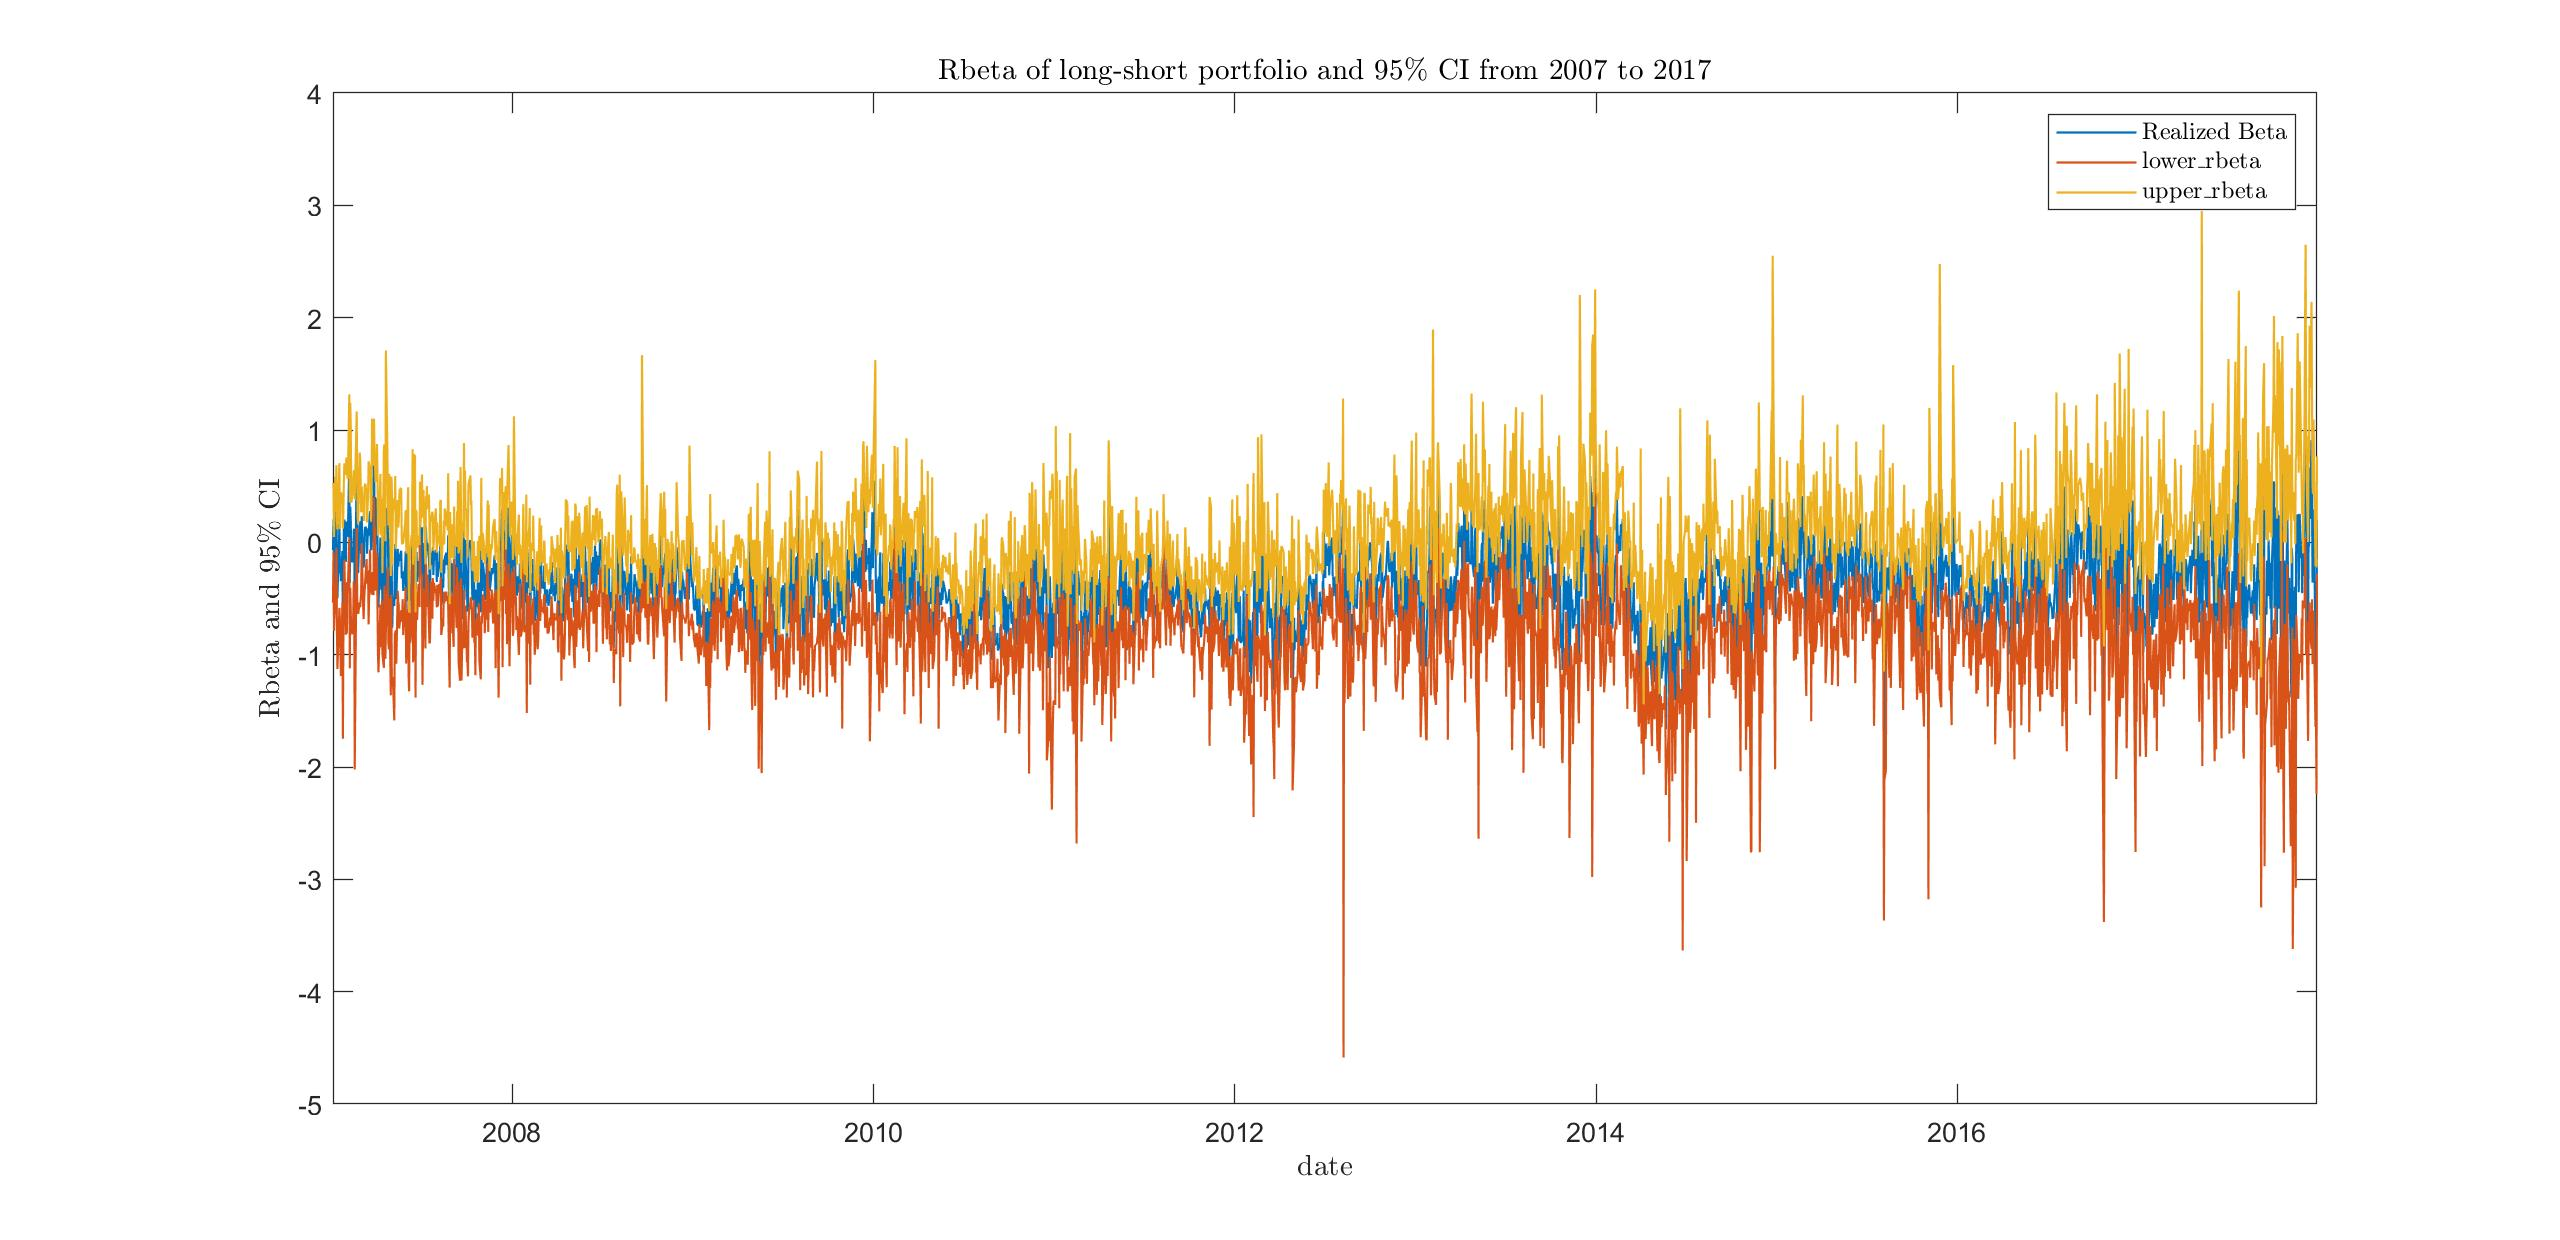
\includegraphics[width=10cm]{figures/q2_c.jpg}
            \centering
            \caption{R$\beta$ and estimated CI of long-short portfolio from 2007 to 2017}
\end{figure}

From this figure we can see most of the value of long-short portfolio concentrate on zero, which means this portfolio may show the character of market neutral. However, there exists some periods that the absolute values of realized beta are large: around 2010, 2013, 2014 and 2017, which are consistent with financial crisis. This discover may be an evidence to support the hypnosis that stocks correlation to market may increase during crisis. \\


  
%----d-----
\item 
The follow is the figure of realized beta and estimated CI of long-short portfolio in October 2008: 
\begin{figure}[H]
           \centering
            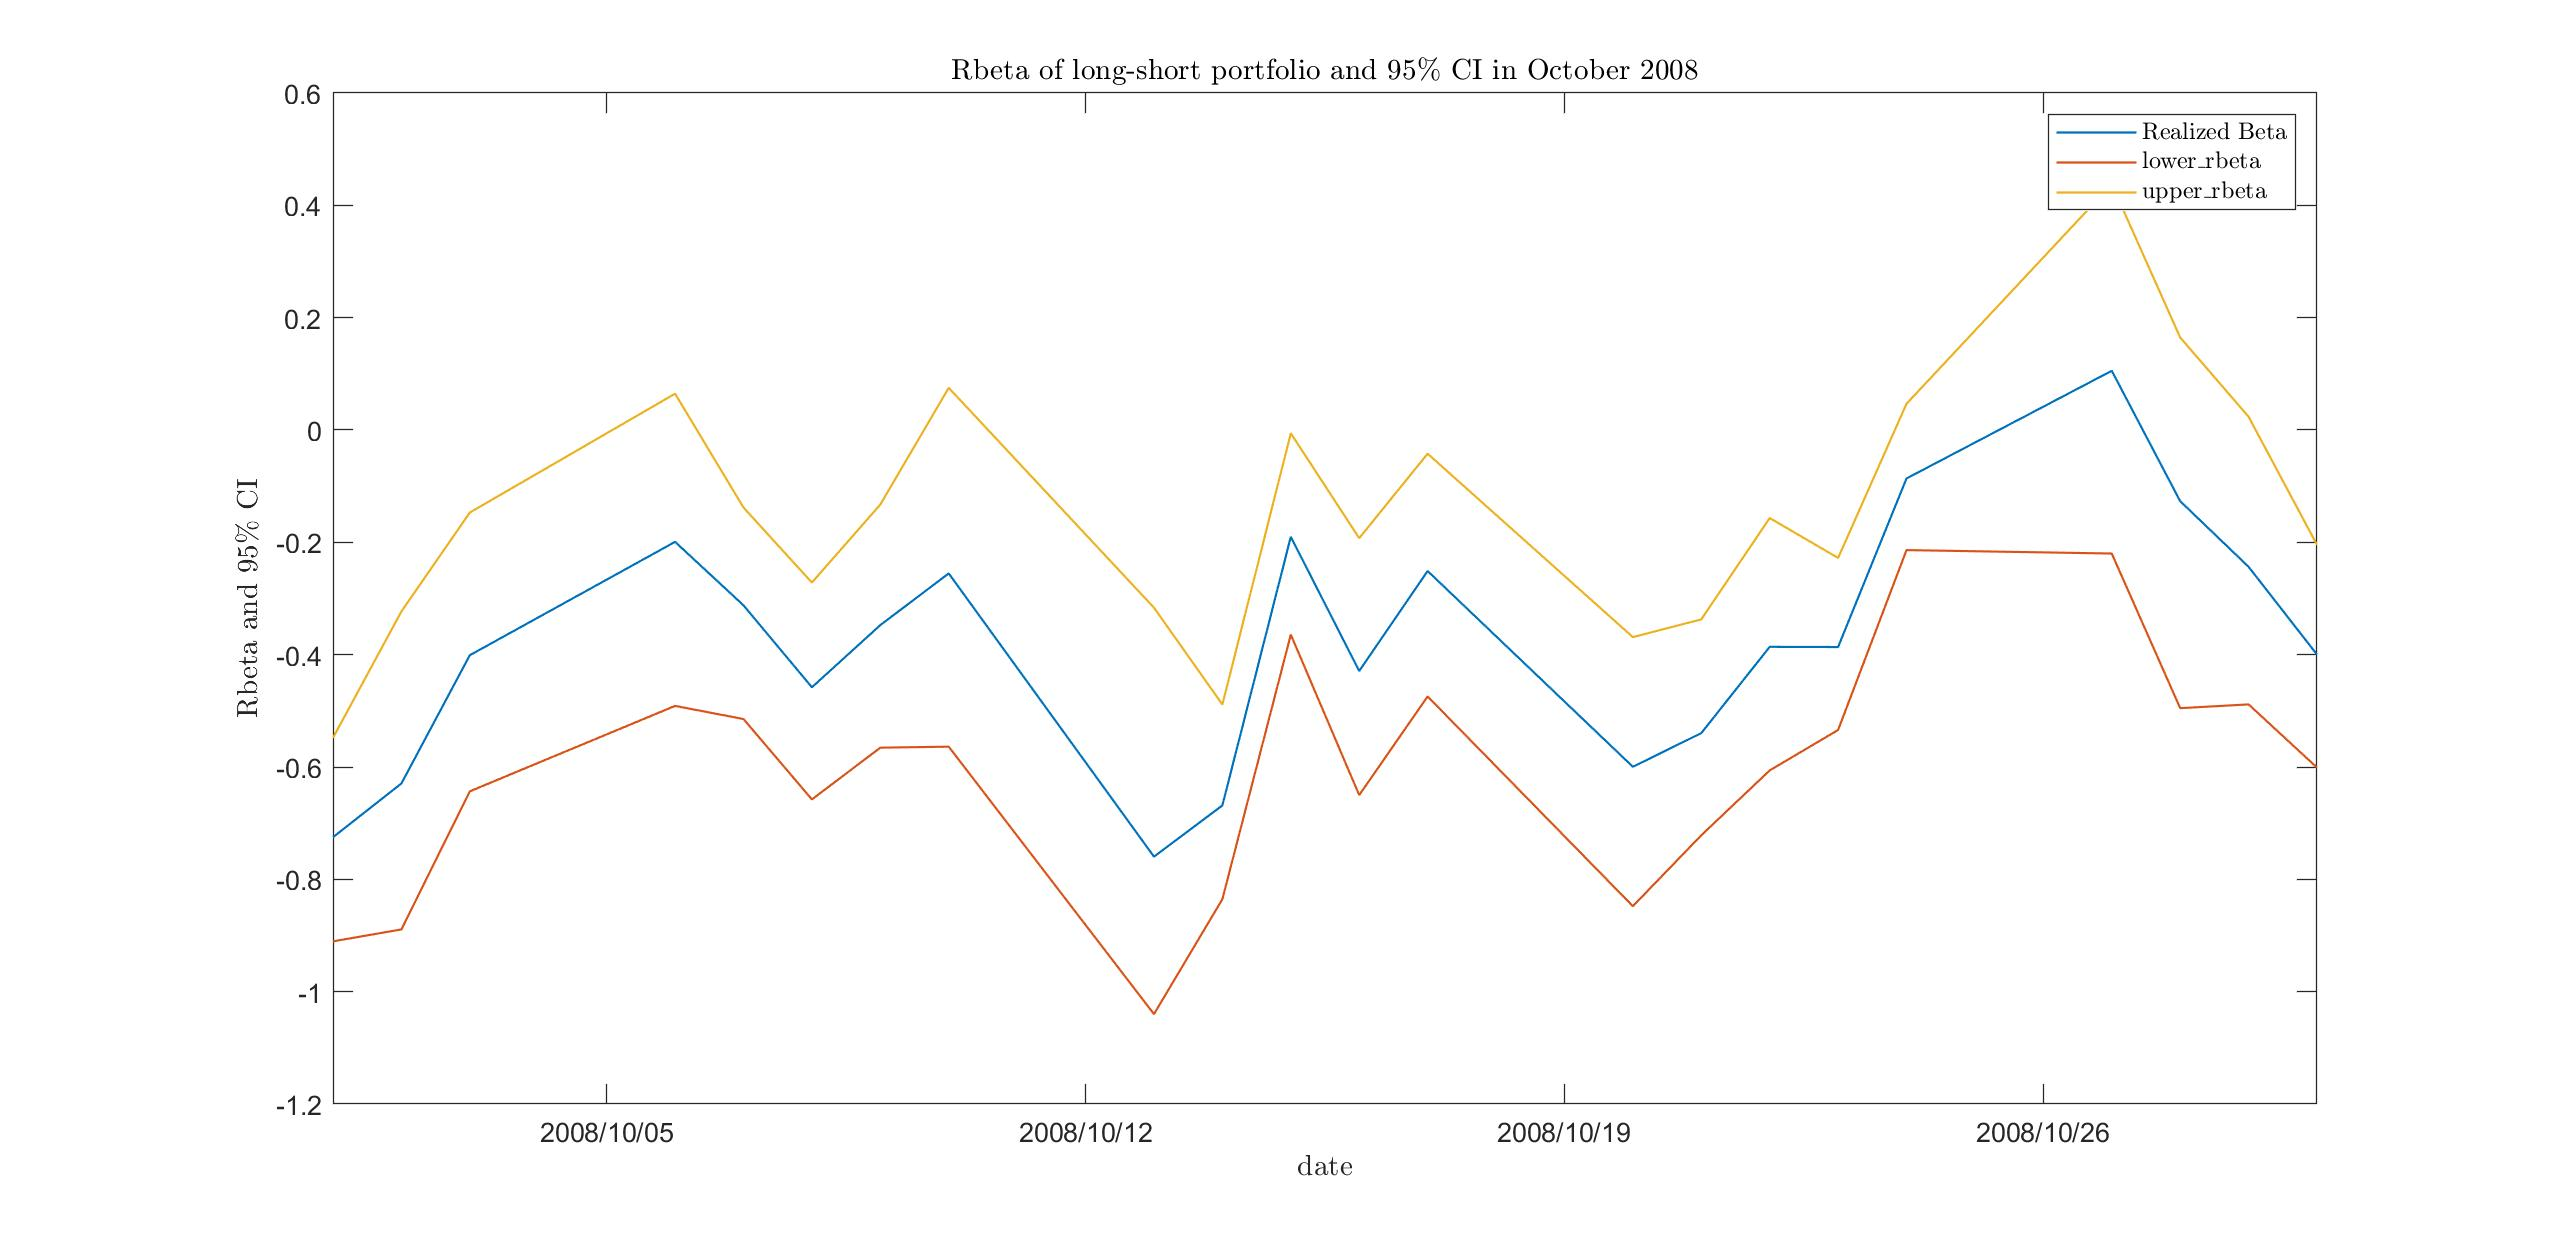
\includegraphics[width=10cm]{figures/q2_d.jpg}
            \centering
            \caption{R$\beta$ and estimated CI of long-short portfolio in October 2008}
\end{figure}
From this figure we can find the confidence interval estimated by bootstrap is good for this specific period: all the observation data fall  into the region bounded by lower confidence interval and upper confidence interval. However, the range of confidence interval width in this period is 0.15-0.6, which means the confidence interval here is not precise enough for most application. \\

As for the value of confidence interval and realized beta, we can see that about 80\% of observations and the estimated confidence intervals are below 0, which means this new portfolio may not be market neutral and it shows negative correlation to market, though this correlation is not weak (most of the absolute value of realized beta is larger than 0.3).\\

%-----part E
\item
To better estimate whether this new portfolio is market neutral or not, we calculate the number of confidence intervals that contains 0.

\begin{table}[ht]
\centering % used for centering table
\begin{tabular}{lcc} % centered columns (4 columns)
\hline\hline %inserts double horizontal lines
\multicolumn{3}{c}{Summary Statistics of confidence interval}\\ [0.5ex]%inserts table
\hline Types & Number & Percentage(\%)\\
%heading
\hline
Do not reject $H_0:R\beta=0$ ($0 \in CI$) & 1352 & 48.8263 \\
Reject $H_0$ and in favor of $R\beta>0$ ($CI_{low}$>0) & 16 & 0.5778\\
Reject $H_0$ and in favor of $R\beta>0$ ($CI_{up}$<0) & 1401 & 50.5959 \\
\hline %inserts single line
\end{tabular}
\end{table}

According to the statistical summary table of confidence interval, we can see that the number of confidence intervals contain 0 is 1352 and takes up 48.8263\% of total sample. This result is not enough for us to reach a conclusion that this new portfolio is market neutral even though the figure shows some clues. \\

The \textbf{MATLAB} code:
   \lstinputlisting{scripts/Question2.m}

\newpage
\end{enumerate}

%---------------------------------------------

\section*{Exercise 3}
  \begin{enumerate}[label=\textbf{(\Alph*)}]
%part 1
\item 
The follow is the statistic summary table of continuous return of PG,DIS and SPY.
\begin{table}[ht]
\centering % used for centering table
\begin{tabular}{cccccc} % centered columns (4 columns)
\hline\hline %inserts double horizontal lines
\multicolumn{6}{c}{Summary Statistics for Continuous Returns}\\ [0.5ex]%inserts table
\hline Stock & Average & Min & 5\% Percentile & 95\% Percentile & Max\\
%heading
\hline
PG & $5.4237\times 10^{-6}$ & -0.0254 & -0.0015 & 0.0016 & 0.0420\\
DIS & $4.3967\times 10^{-6}$ & -0.0323 & -0.0022 & 0.0022 & 0.0474\\
SPY & $1.7039\times 10^{-6}$ & -0.0293 & -0.0015 & 0.0015 & 0.0376\\
\hline %inserts single line
\end{tabular}
\end{table}

%-----part B
\item The number of detected jumps in the market is 116.
%---part C
\item The follow is the statistic summary table of realized beta of PG and DIS:
\begin{table}[ht]
\centering % used for centering table
\begin{tabular}{cccccc} % centered columns (4 columns)
\hline\hline %inserts double horizontal lines
\multicolumn{6}{c}{Summary Statistics of Realized Beta}\\ [0.5ex]%inserts table
\hline Stock & Average & Min & 5\% Percentile & 95\% Percentile & Max\\
%heading
\hline
PG & 0.5403 & -0.4167 & 0.1472 & 0.9709 & 2.0421\\
DIS & 0.9312 & -1.0811 & 0.4731 & 1.3581 & 2.8132\\
\hline %inserts single line
\end{tabular}
\end{table}

%---part D
\item 
Here are the figures of realized beta of PG and DIS from 2007 to 2017.
\begin{figure}[H]
           \subfigure{
           \begin{minipage}[l]{1\linewidth}
           \centering
            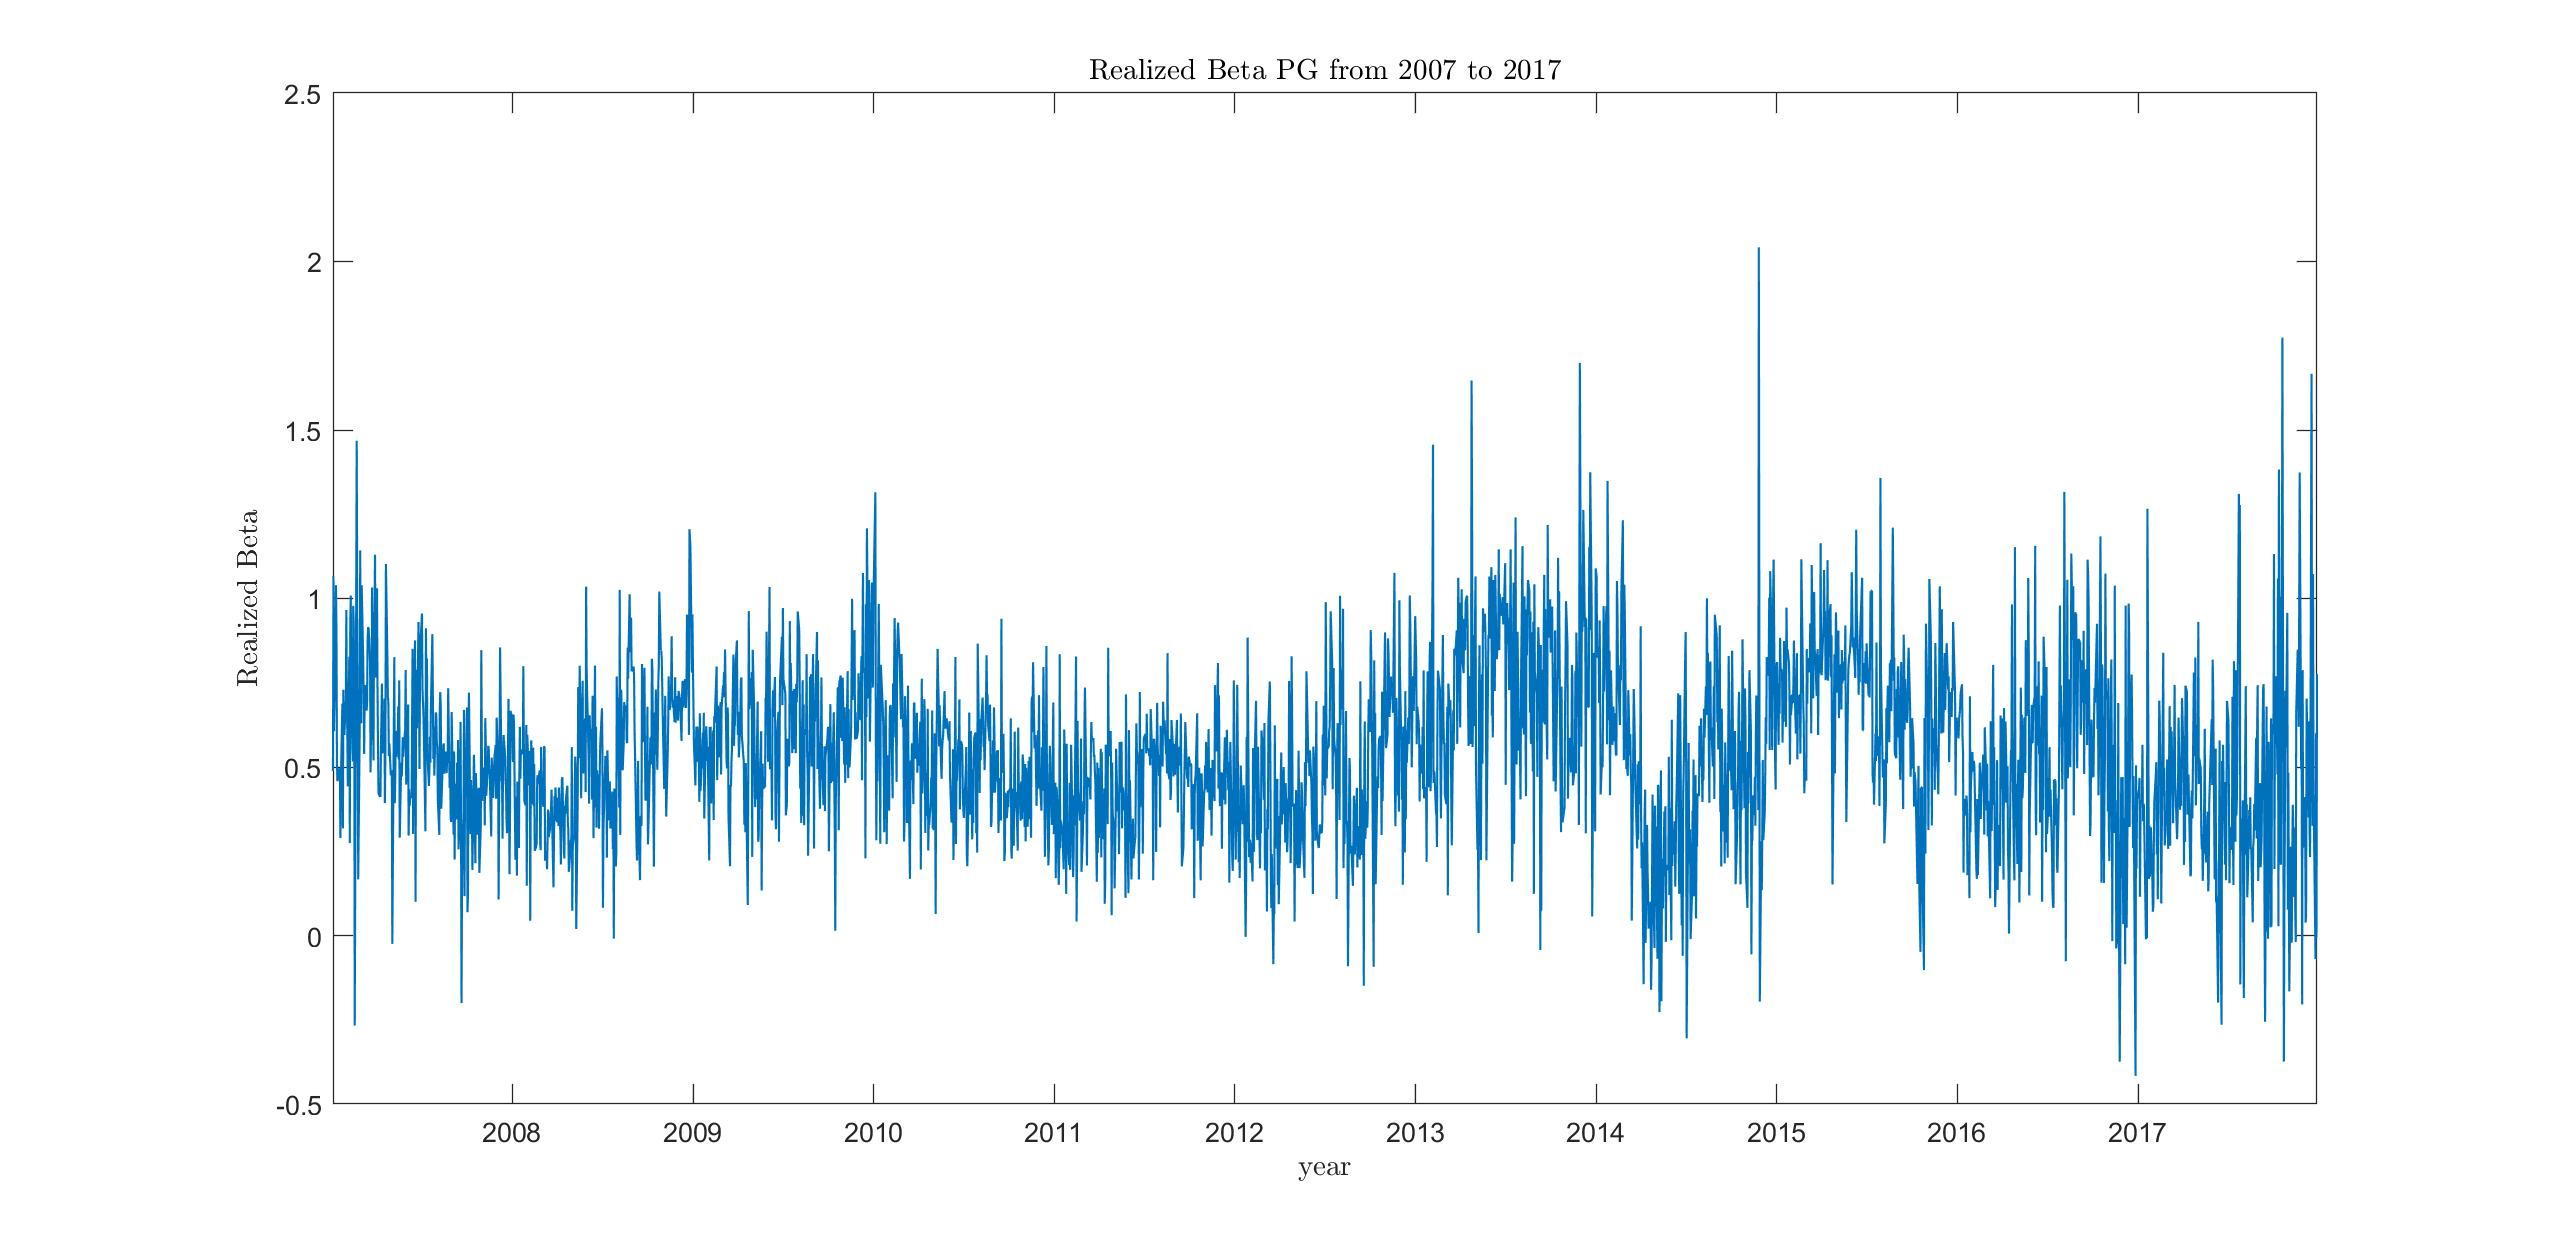
\includegraphics[width=3in]{figures/q3_d_PG.jpg}
            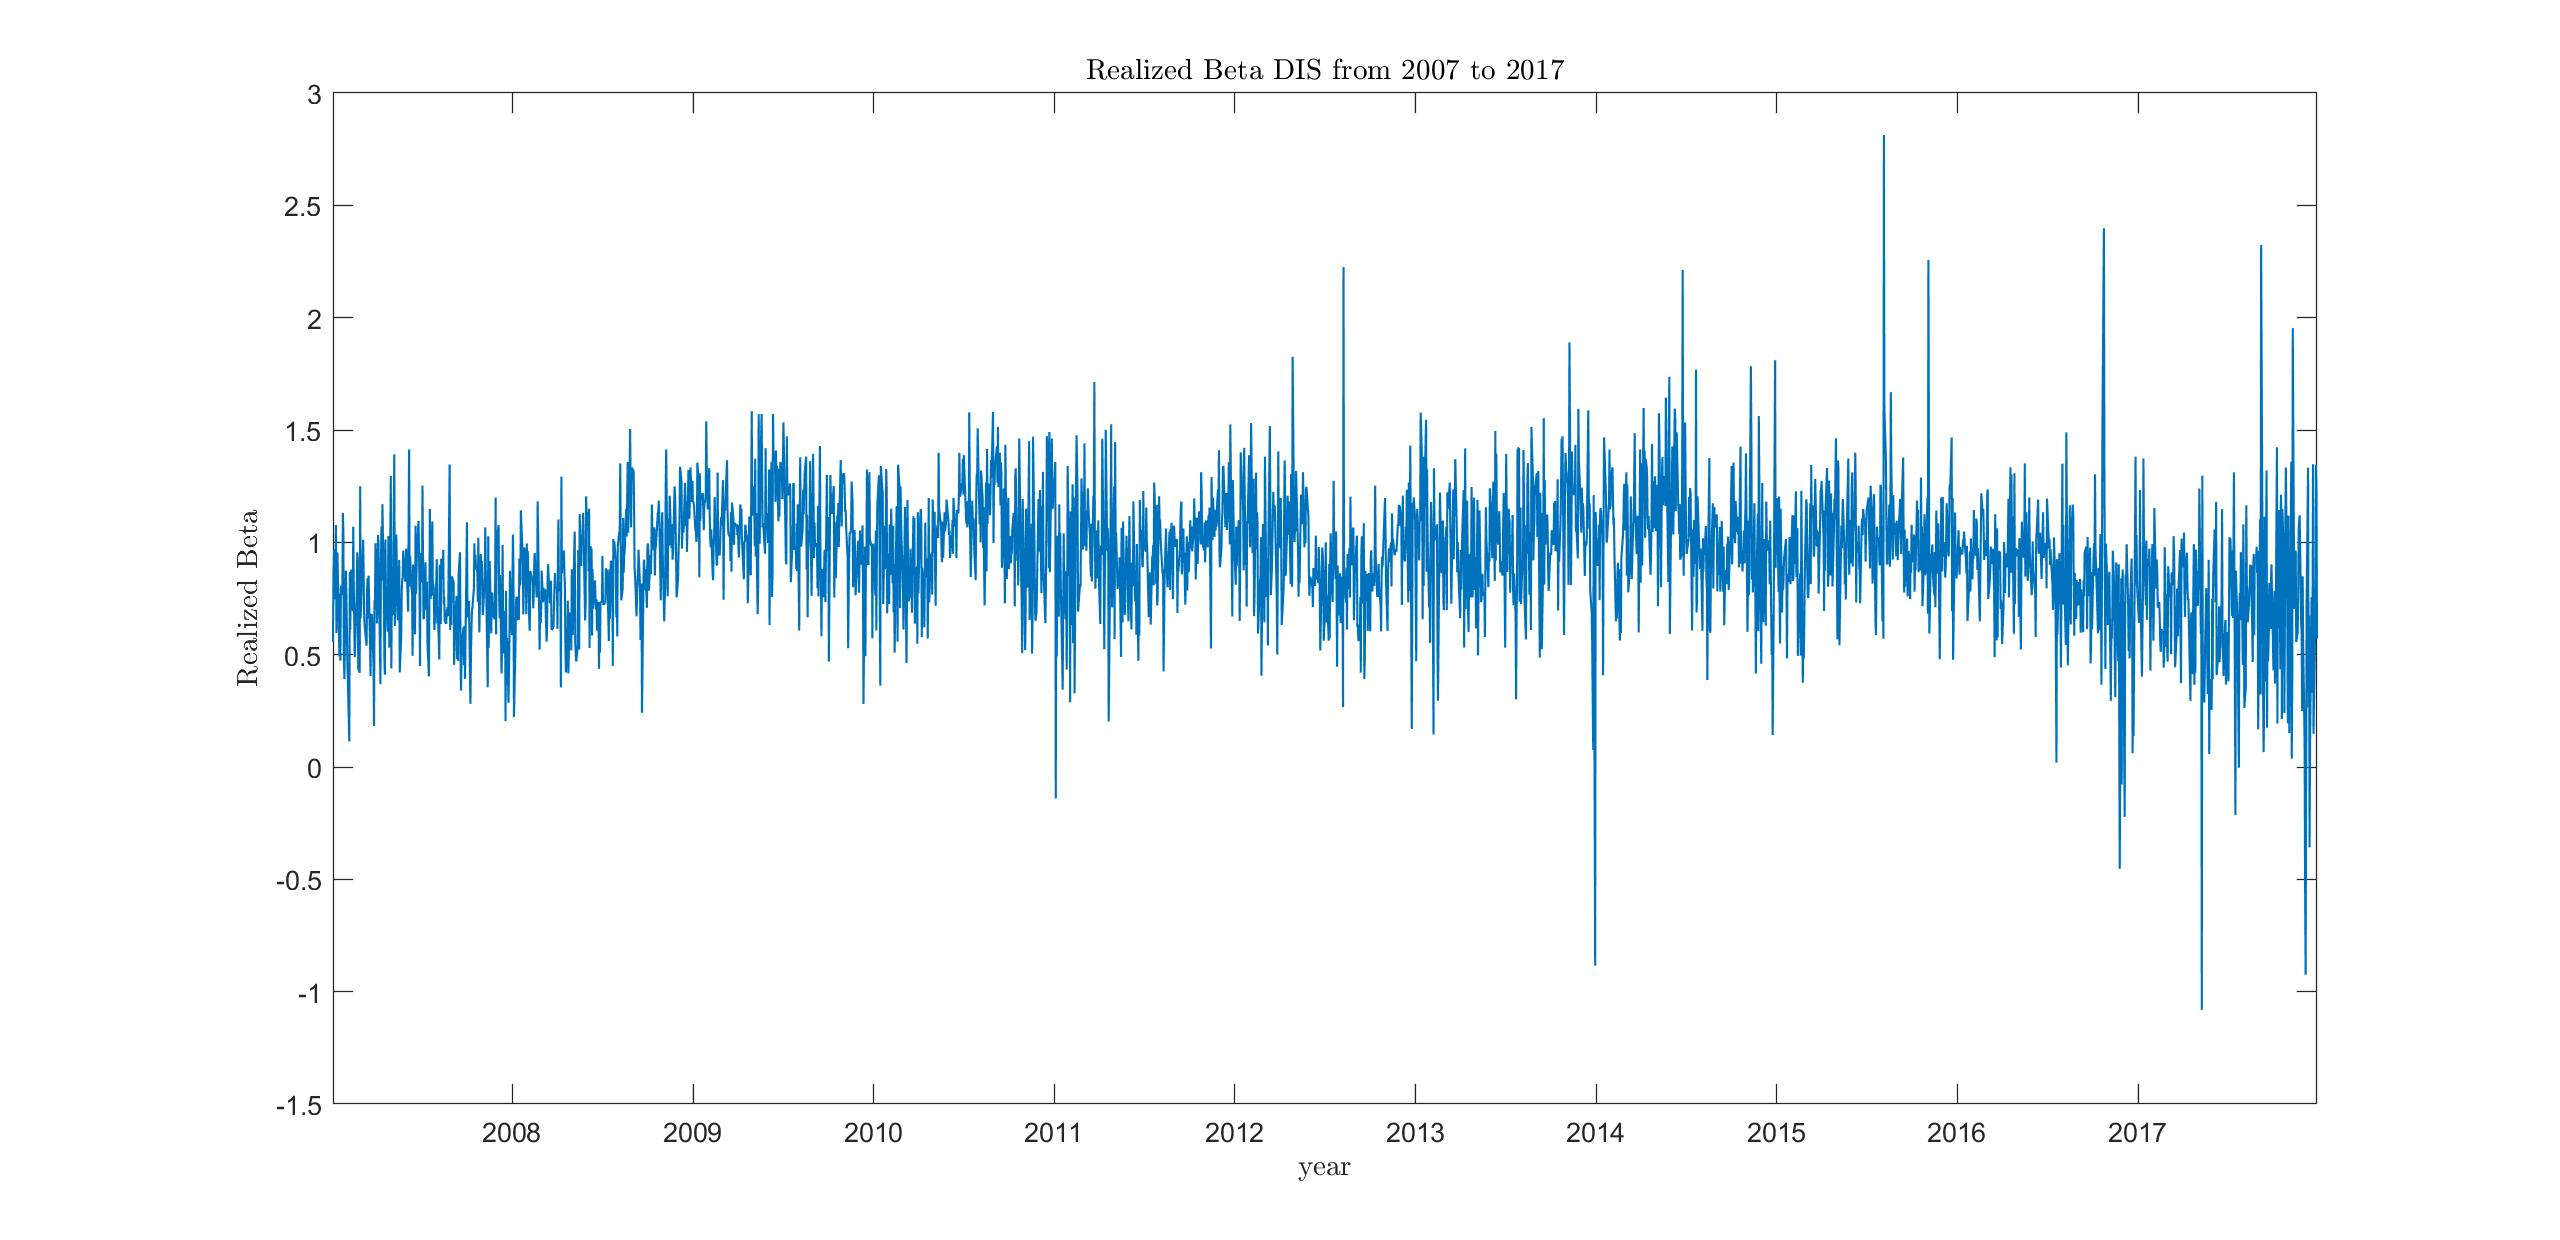
\includegraphics[width=3in]{figures/q3_d_DIS.jpg}
            \end{minipage}
            }
            \centering
            \caption{Realized beta and its estimated confidence interval of PG and DIS}
\end{figure}
From the figures, PG’s realized beta mostly falls below the line $R\beta$= 1, which means that PG may have a lower beta than the market for most in trading day. The situation is different in the case of DIS. As we can see from the figure, most of DIS’ realized beta falls above or around the line $R\beta$= 1, this indicates that the beta of DIS may have a higher or equal value to the market's in most of trading day.\\

We can do some statistical work to support our viewpoint. Here is the summary table of estimated realized beta for PG and DIS.

\begin{table}[ht]
\centering % used for centering table
\begin{tabular}{clcc} % centered columns (4 columns)
\hline\hline %inserts double horizontal lines
\multicolumn{4}{c}{Summary Statistics of confidence interval}\\ [0.5ex]%inserts table
\hline Stock& Types & Number & Percentage(\%)\\
%heading
\hline
 & $CI^{l}>1$ & 2 & 0.0722\\ 
PG &$1 \in CI$ & 665 & 24.0159 \\
& $CI_{u}<1$ & 2102 & 75.9119 \\
\hline
 & $CI^{l}>1$  & 204 & 7.3673\\
DIS&$0 \in CI$ & 2100 & 75.8397 \\
& $CI_{u}<1$  & 465 & 16.7930 \\
\hline %inserts single line
\end{tabular}
\end{table}

For PG stock, the number of confidence interval below 1 takes up 75.91\%, which indicates PG stock will probably have a lower beta than the market for most of its trading day. A lower beta value means that the stock is less volatility than the market and has a lower risk and returns. For DIS stock, the number of confidence interval contain 1 takes up 75.84\%, which indicates DIS stock will probably have a equal beta with the market for most of its trading day. The beta value equals to market beta means that the stock has the same volatility with the market.


%---part e
\item The follow is the statistic summary table of realized beta of PG and DIS:
\begin{table}[ht]
\centering % used for centering table
\begin{tabular}{ccccc} % centered columns (4 columns)
\hline\hline %inserts double horizontal lines
\multicolumn{5}{c}{Summary Statistics of Residual Correlation}\\ [0.5ex]%inserts table
\hline  Average & Min & 5\% Percentile & 95\% Percentile & Max\\
%heading
\hline
0.0186 & -0.4993 & -0.2443 & 0.2881 & 0.5563\\
\hline %inserts single line
\end{tabular}
\end{table}

According to this table, the correlation of PG and DIS' residual PG and DIS is really small, which means that the stock returns for both stocks are mostly explained by the market factor and they are not very related to each other.\\

%---part F
\item Here is the figure of correlation and its 95\% estimated confidence interval.

\begin{figure}[H]
           \centering
            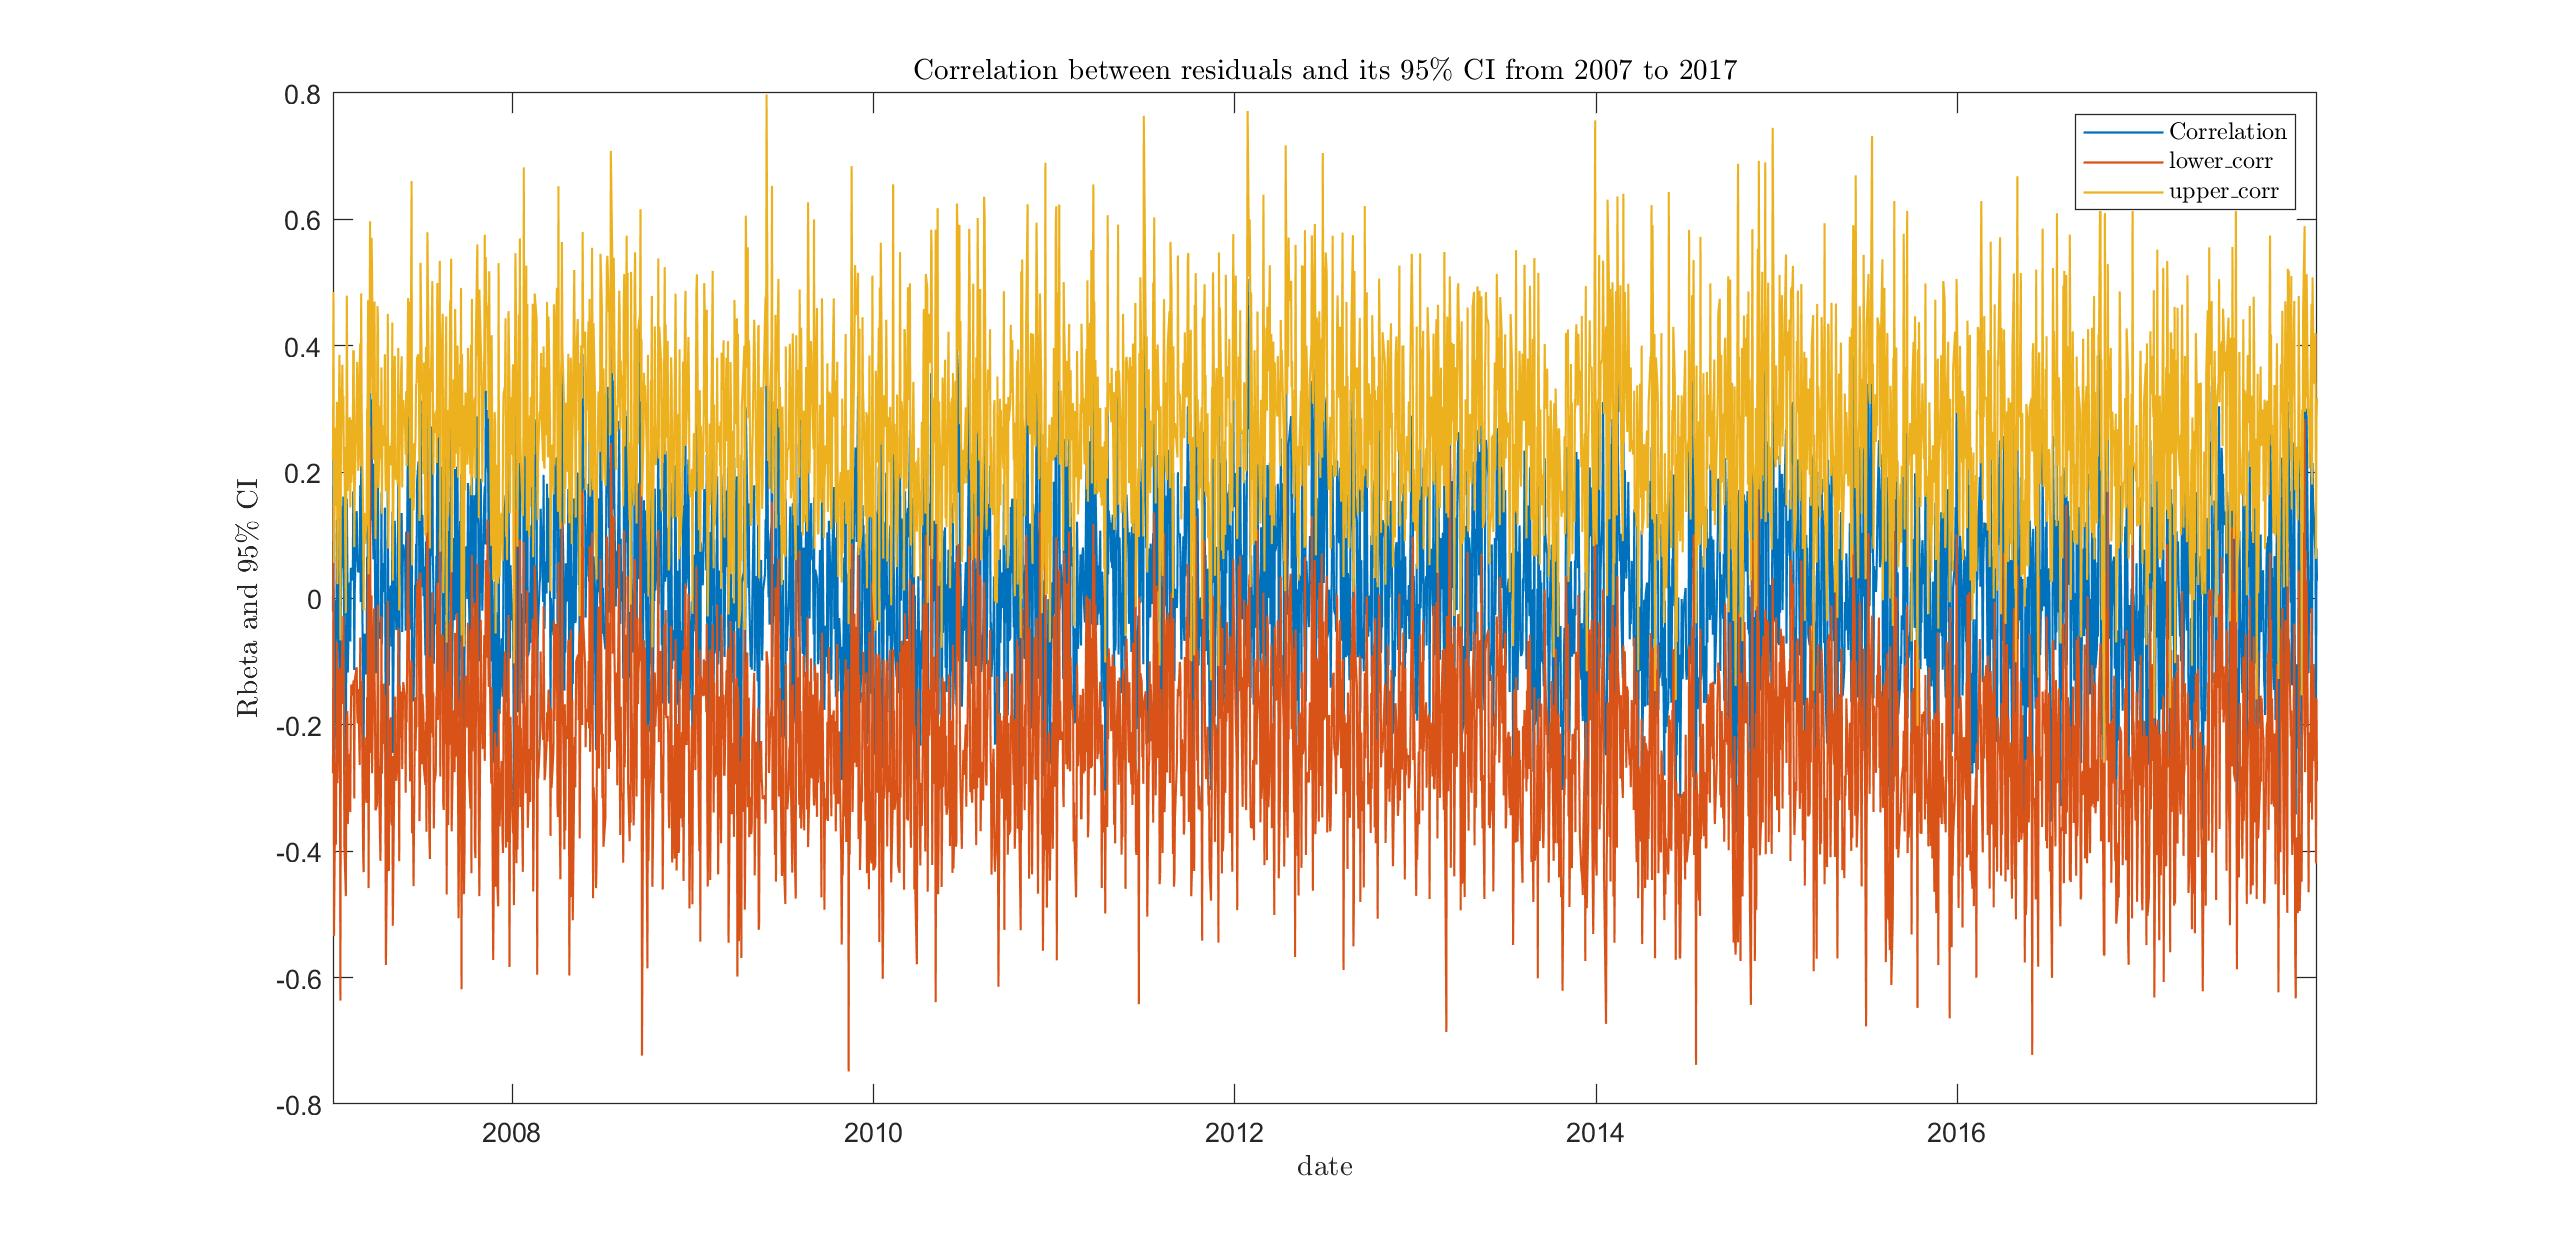
\includegraphics[width=10cm]{figures/q3_f.jpg}
            \centering
            \caption{Correlation and its 95\% CI from 2007 to 2017}
\end{figure}

From the figure we can see the correlations between two residuals are concentrated on zero and most of the confidence intervals have covered value zero, which means the linear relation between this two residuals is weak. Since these residuals are produced by removing the common movement with market from their log-returns, the weak linear relationship between residuals may indicate that these two stocks do not share other common movements except the market co-movement.\\




%---part G
\item Here is the figure of correlation and its 95\% estimated confidence interval for October 2008.
\begin{figure}[H]
           \centering
            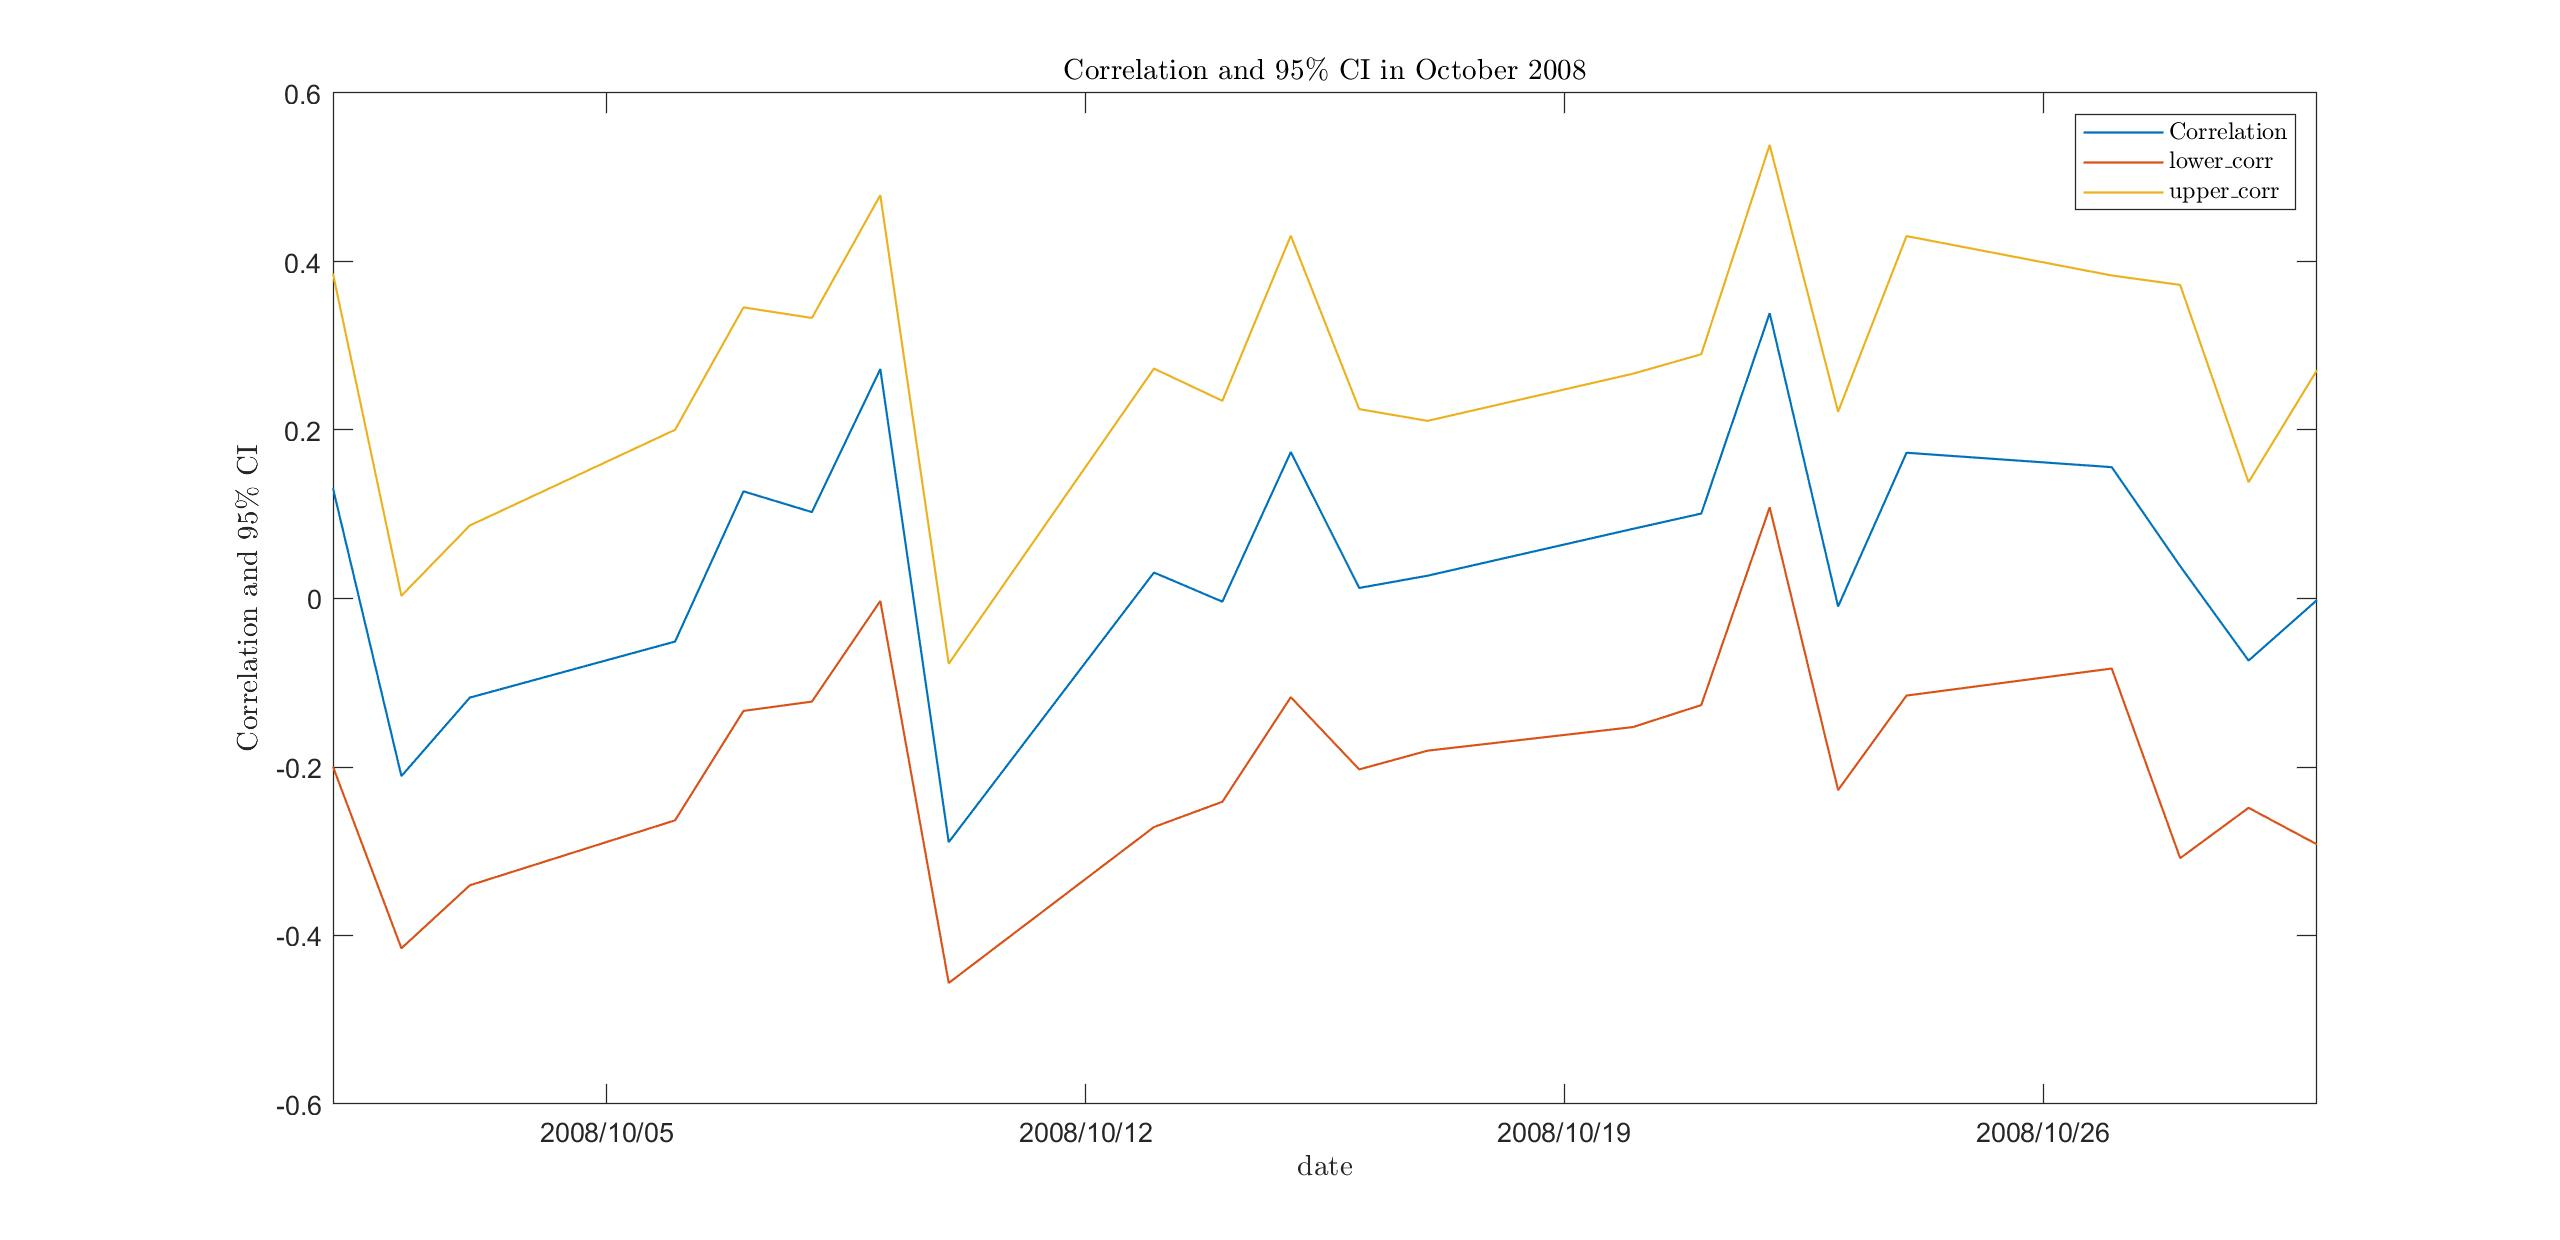
\includegraphics[width=10cm]{figures/q3_g.jpg}
            \centering
            \caption{Correlation and its 95\% CI for October 2008}
\end{figure}

According to the figure, the range of correlation between residuals is (-0.3, 0.3) and most of them are moving within (-0.1, 0.1). This indicates that the correlation is weak between these to variables. As for the confidence interval, the width is in the range of (0.1, 0.5), the max and min value of confidence interval is 0.5 and -0.4 respectively. From these data we can see that the possible correlation between the residuals will not be very strong, it is reasonable to reach the conclusion that the two stocks do not share other common movements except for the market movement.


%---part H
\item To better understand the correlation between residuals, we calculate the number of correlation confidence intervals that contains 0.

\begin{table}[ht]
\centering % used for centering table
\begin{tabular}{lccc} % centered columns (4 columns)
\hline\hline %inserts double horizontal lines
\multicolumn{4}{c}{Summary Statistics of confidence interval}\\ [0.5ex]%inserts table
\hline Types & Number & Percentage(\%) & ``p''\\
%heading
\hline
Do not reject $H_0:\rho_{et}{=}0$: & 2501 & 90.3214 & $p_0$=9.9246\\
Reject $H_0$ and in favor of $\rho_{et}>0$ & 168 & 6.0672 & $p_+$=0.6667\\
Reject $H_0$ and in favor of $\rho_{et}<0$ & 100 & 3.6114 & $p_-$=0.3968 \\
\hline %inserts single line
\end{tabular}
\end{table}

According to the statistical summary table of confidence interval, we can see that the number of confidence interval that contain 0 is 2501 and takes up 90.3214\% of total sample. And the $p_0$ value here represent the possible number of years in our data that the two stock do not have other co-movements except the market movements. As we can see that, from total observe time length (2007 to 2017), the number of year can not reject $\rho_{et}=0$ is 9.92, that is for most of our observation, the correlation of residuals is near to zero. All these results support us to reach a conclusion that these two stocks do not have other common movements. \\



The \textbf{MATLAB} code:
   \lstinputlisting{scripts/Question3.m}
\end{enumerate}
\newpage


\end{document}
